\documentclass[10pt,a4paper]{article}
\usepackage[utf8]{inputenc}
\usepackage{amsmath}
\usepackage{amsfonts}
\usepackage{amssymb}
\usepackage{tikz}
\usepackage{graphicx}
\author{James Lee}
\title{11th Assignment of Computational Physics}
\begin{document}
	\maketitle
	\begin{abstract}
		In this report I present to you the numerical solution to Problem 4.11.
	\end{abstract}
	\section{Introduction}
	The precession of the perihelion of Mercury is one of the three earliest experimental test of GR. It is well known to astronomers that Mercury's perihelion is precessing at a considerable rate. Physicists prior to Einstein had investigated this precession using Newtonian mechanics. After they had taken into accounts of pertubations of planets near Mercury, they found that such pertubations could not be the whole story, for there existed an extra $43\text{ arcseconds/century}$ precession rate.\\
	After having proposed the theory of general relativity, Einstein showed that general relativity agrees closely with the observed amount of perihelion shift. This was a powerful factor motivating the adoption of general relativity.\\
	In general relativity, spacetime near the Sun is described by Schwarzschild metric:
	\begin{equation}
     d^{2}l=-(1-\frac{2M}{r})d^{2}t+(1-\frac{2M}{r})^{-1}d^{2}r+r^{2}d^{2}\Omega
    \end{equation}
	Mercury moves along the geodesics associated with this metric.\\
	Geodesics are determined by geodesics equation:
	\begin{equation}
	 \frac{d^{2}x^{\mu}}{d\tau^2}+\Gamma^{\mu}_{\sigma \nu}\frac{dx^{\sigma}}{d\tau}\frac{dx^{\nu}}{d\tau}=0
	\end{equation}
	where $\Gamma^{\mu}_{\sigma \nu}$ is the Christoffell symbols related to the metric $g_{\mu \nu}$.
	Detailed examinations show that Mercury's precession rate is described by the following formula (R.Wald):
	\begin{equation}
	\omega_p=\frac{3(GM)^{3/2}}{c^2(1-e^2)a^{5/2}}
	\end{equation}
	Numerical result shows that $\omega_p=43\text{ arcseconds/century}$, which is precisely the observed rate!\\
	In the following sections, I will use numerical methods to study the subject.
    \section{Main Content}
    \subsection{Mercury's Motion}
    The modified gravity law is:
    \begin{equation}
    F_{G}=\frac{GM_SM_M}{r^2}(1+\frac{\alpha}{r^2})
    \end{equation}
    In order to solve the motion of Mercury, I will use Euler-Cromer method to do this numerically.\\
    A crucial subject is to set the appropriate initial condition:
    \begin{align}
    x|_{t=0}&=0.47\text{ AU}\\
    y|_{t=0}&=0\\
    v_x|_{t=0}&=0\\
    v_y|_{t=0}&=8.2\text{ AU/Yr}
    \end{align}
    With the dynamical equations and initial conditions in hands, one can easily obtain the orbit.\\
    \begin{figure}[htbp]
    	\centering
    	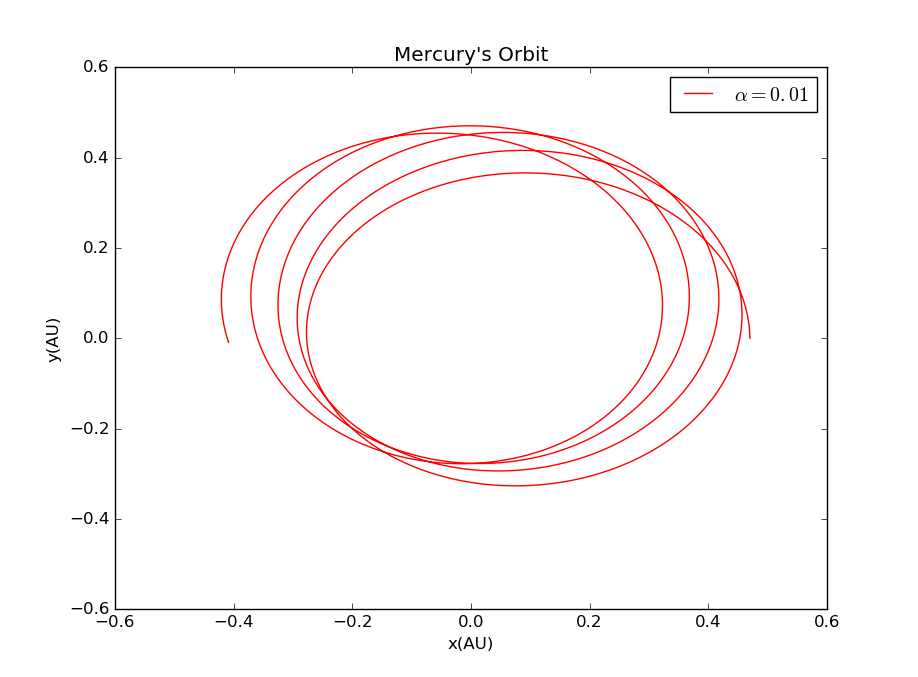
\includegraphics[width=5in]{Mercury_1.png}
    	\caption{Mercury's Orbit with $\alpha=0.01$}
    \end{figure}
    I should remark that this plot has adopted a large $\alpha$ in order to make precession visible in the plot.\\
    As we can see in the plot, Mercury's orbit is indeed precessing due to GR effects.\\
    How fast is this precession? In fact, using numerical methods, one can show that this precession is linear with time.\\
    \begin{figure}[htbp]
    	\centering
    	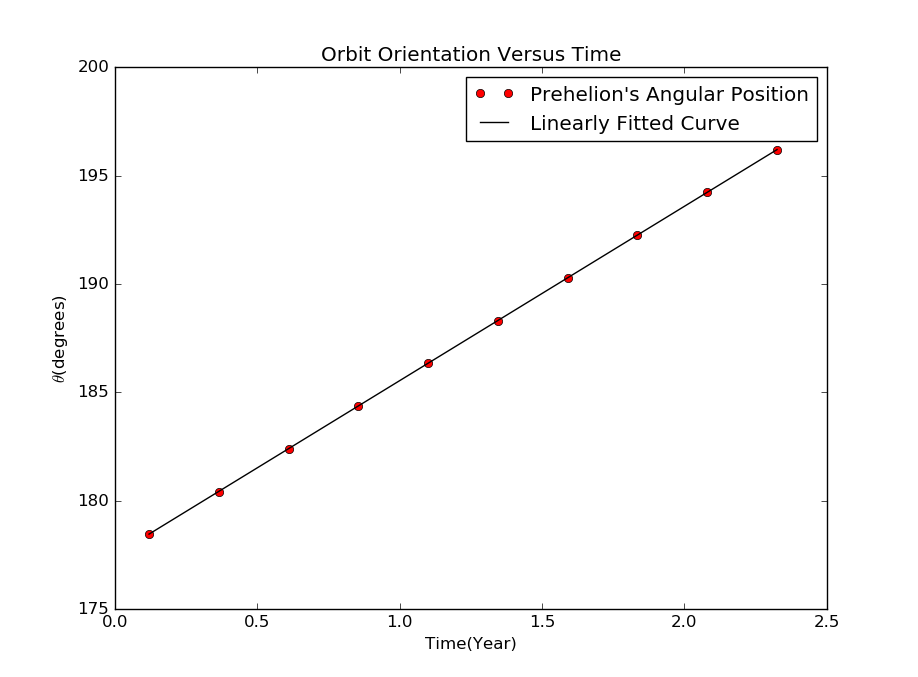
\includegraphics[width=5in]{Mercury_2.png}
    	\caption{Orbit Orientation versus Time with $\alpha=0.0008$}
    \end{figure}
    Regression analysis shows that in $\alpha=0.008$ case, we have:
    \begin{equation}
    \frac{d\theta}{dt}=8.044\text{ Degrees/Yr}
    \end{equation}
    What about other $\alpha$? As we know, the real $\alpha=1.1\times 10^{-8}\text{ AU}^2$. I investigated several cases and found the following result in figure.3.\\
    As we can see in the plot, the precession rate is linear with $\alpha$. 
    \begin{equation}
    \frac{d\theta}{dt}=C\alpha
    \end{equation}
    Regression results show that:
    \begin{equation}
    C=1.12\times 10^{4}
    \end{equation}
    This result enables us to calculate the precession rate of perihelion of Mercury:
    \begin{align}
    \omega_p&=1.1\times 10^{-8}\times 1.12\times 10^{4}\\
    &=1.2\times 10^{-4}\text{ Degrees/Yr}\\
    &=43\text{ arcseconds/century}
    \end{align}
    which is in accord with experimental results. 
    \begin{figure}[htbp]
    	\centering
    	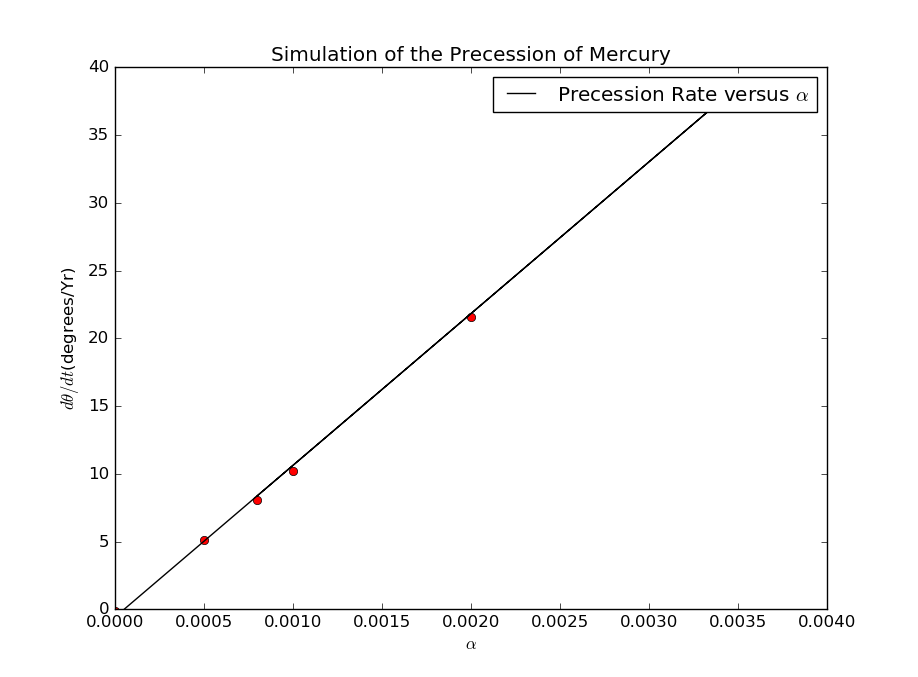
\includegraphics[width=5in]{Mercury_3.png}
    	\caption{Precession Rate versus $\alpha$}
    \end{figure}
    
    \subsection{Precession and Eccentricity}
    In the following figures I will plot Mercury's motion with different eccenricity(different initial conditions):\\
    \begin{figure}[htbp!]
    	\centering
    	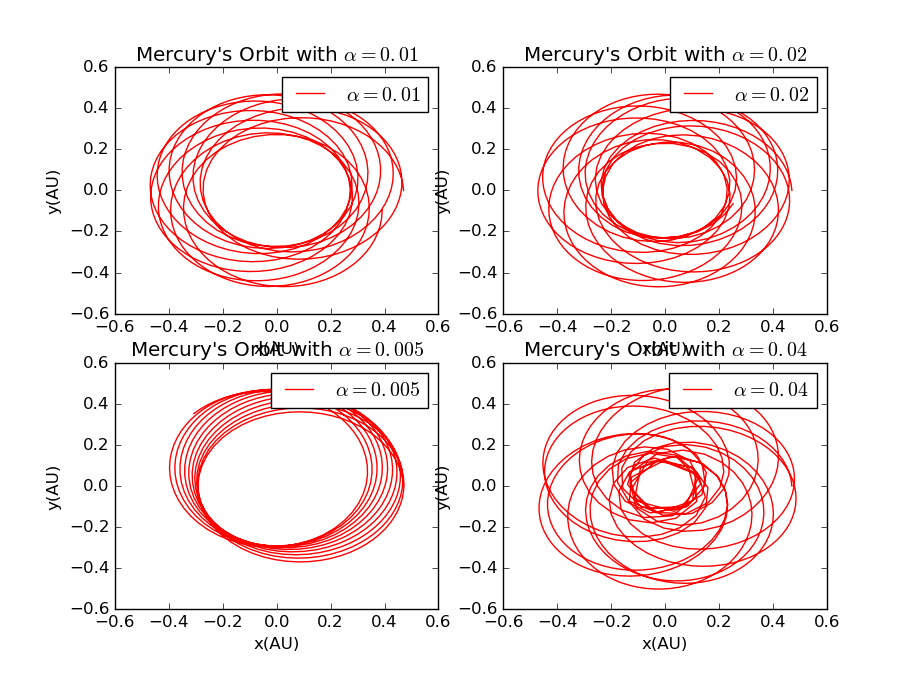
\includegraphics[width=3in]{Mercury_4.png}
    	\caption{Mercury's Motion with $e=0.206$}
    \end{figure}
    \begin{figure}[htbp!]
    	\centering
    	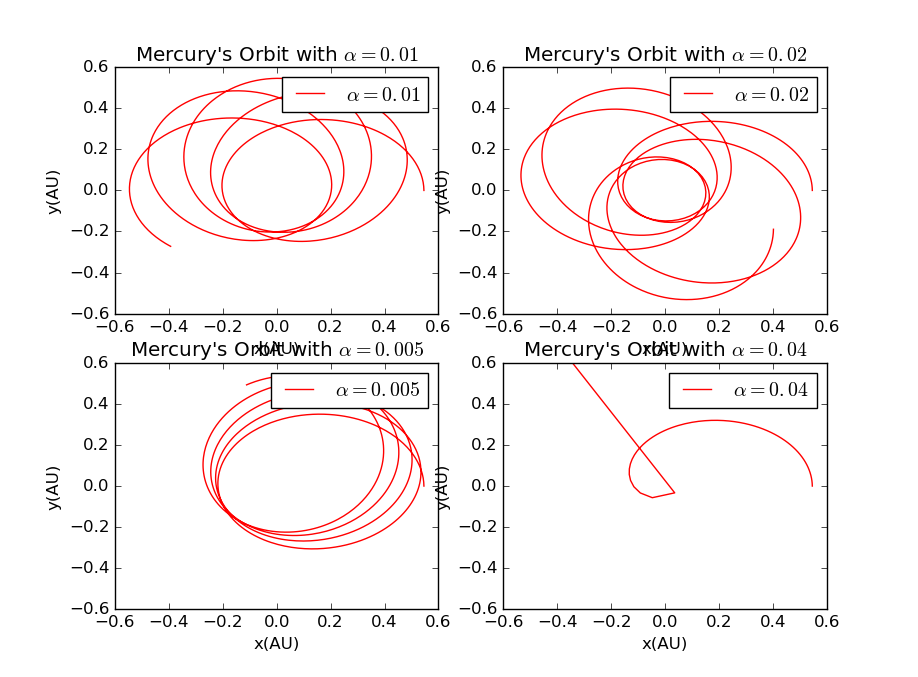
\includegraphics[width=3in]{Mercury_5.png}
    	\caption{Mercury's Motion with $e=0.4$}
    \end{figure}
    \begin{figure}[htbp!]
    	\centering
    	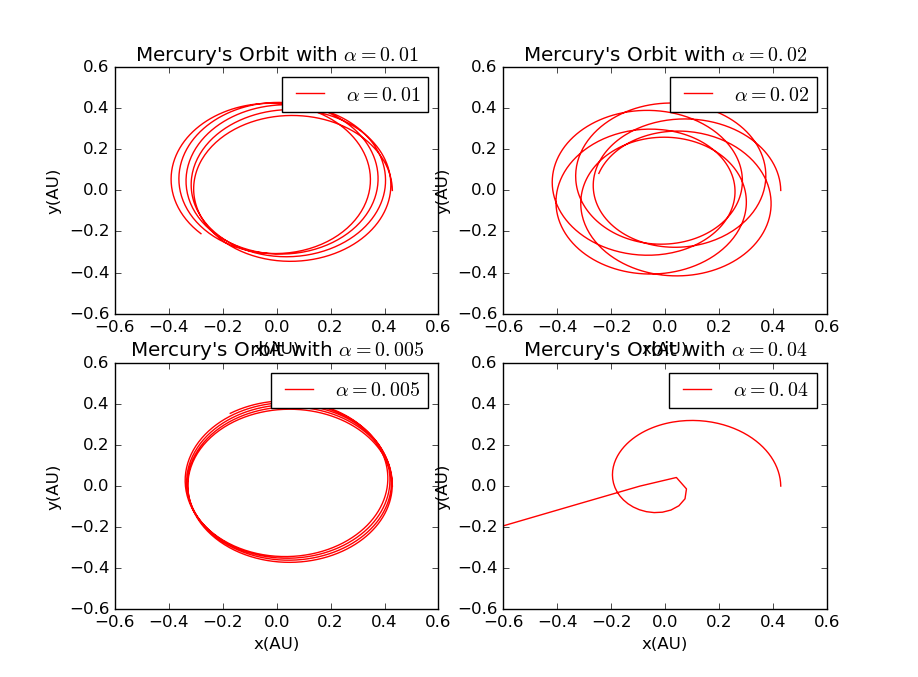
\includegraphics[width=3in]{Mercury_6.png}
    	\caption{Mercury's Motion with $e=0.1$}
    \end{figure}
    \begin{figure}[htbp!]
    	\centering
    	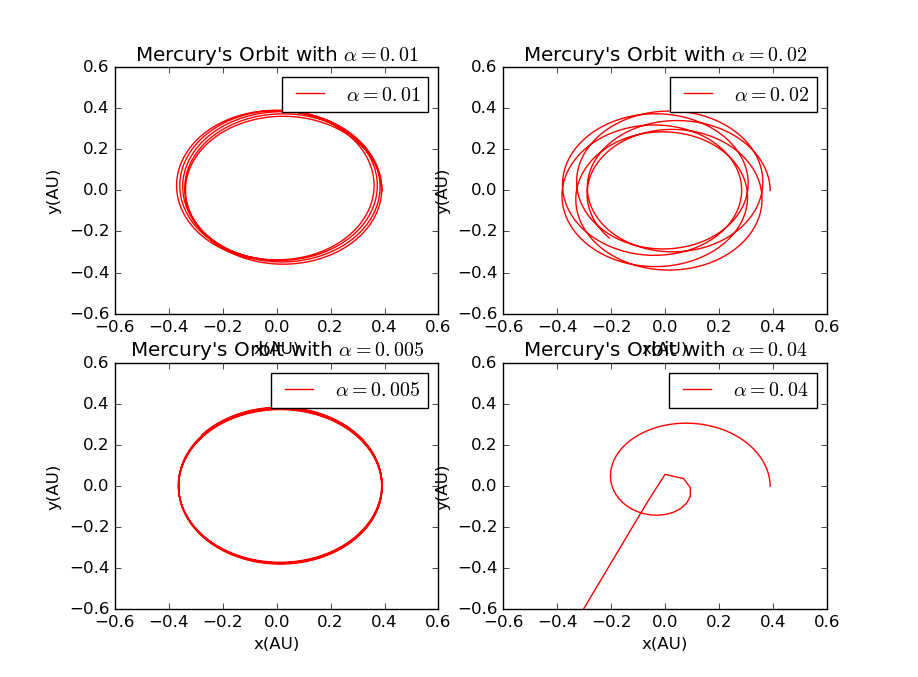
\includegraphics[width=3in]{Mercury_7.png}
    	\caption{Mercury's Motion with $e=0$}
    \end{figure}
    There are several amazing facts that are shown in the plots:\\
    1. When $\alpha$ is large, i.e. general relativity effects are extraodinary, there may not be a close curve regardless of what the initial conditions are.\\
    2. Even when the orbit is circular, precessions still exist.
    
    \begin{thebibliography}{99}
    	\bibitem{}Hunter J, the Matplotlib Documentation, 2016
    	\bibitem{}Giordano N.J, Nakanishi H, Computational Physics, Pearson Education, 2007
    	\bibitem{}Wald, General Relativity, The University of Chicago Press, 1984
    \end{thebibliography}
\end{document}